\documentclass[aps,prd,reprint]{revtex4-1}

\usepackage{hyperref}
\usepackage{amsmath}
\usepackage{amssymb}
\usepackage{graphicx}

\newcommand{\order}[1]{\mathcal{O}\left( #1 \right)}
\newcommand{\fixme}[1]{\textbf{FIXME: #1}}

\newcommand{\xmin}{x_\mathrm{min}}

\DeclareMathOperator{\erf}{erf}

\begin{document}

\title{Bayesian Rate Estimation}

\author{Will M. Farr}
\email{w-farr@northwestern.edu}
%\homepage{http://faculty.wcas.northwestern.edu/will-farr/}
% \affiliation{Center for Interdisciplinary Exploration and Research in Astrophysics (CIERA)\\
% Department of Physics and Astronomy\\
% Northwestern University, 2145 Sheridan Road, Evanston, IL 60208}
\affiliation{Northwestern University and CIERA}

\author{Ilya Mandel}
\email{ilya@chgk.info}
%\homepage{http://www.chgk.info/~ilyamandel/}
% \affiliation{School of Physics and Astronomy\\University of Birmingham\\Edgbaston B15 2TT Birmingham\\United Kingdom}
\affiliation{University of Birmingham}

\author{Jon Gair}

\begin{abstract}
  We show how to obtain a Bayesian estimate of the rate of signal
  events from a set of signal and background events indexed by a
  ranking statistic when the shapes of the signal and background
  distributions are known, can be estimated, or approximated.  We
  focus on the specific application of estimating astrophysical rates
  of the coalescence of compact binary black holes or neutron stars
  from a set of triggers in the LIGO/Virgo gravitational wave
  detectors, but our framework is fully general.  We discuss the
  systematic effects on the rate estimate due to differences between
  the assumed and true shapes of the foreground or background
  distributions, identifying ways these effects can be minimized.
  Similarly, we discuss the effects of various priors on the rate,
  including uninformative priors, weakly-informative priors, and the
  use of priors from previous rate experiments.  In the limit where
  the expected signal rate gives high probability of zero or one
  signal in the data, our technique reduces to the ``loudest event
  statistic,'' but it is generally applicable to arbitrarily large
  signal rates.
\end{abstract}

\maketitle

\section{Introduction}

\fixme{Introduce the necessity of estimating rates, prior work (like
  \cite{Biswas2009}), Bayesian inference.}

\section{Model}

We assume that we are presented with a data set of $N$ events.  Each
event may be due to either a signal of interest or an uninteresting
background.  Each event is associated with a ranking statistic, $x$.
Our data set therefore consists of the ranking statistics for the set
of events:
\begin{equation}
  d = \{ x_i | i = 1, \ldots, N \}.
\end{equation}

We assume that both the foreground and background events are samples
from an inhomogeneous Poisson process with rates (per unit ranking
statistic, $x$)
\begin{equation}
  \frac{dN_f}{dx} = f(x)
\end{equation}
and 
\begin{equation}
  \frac{dN_b}{dx} = b(x).
\end{equation}
The cumulative rates of the two processes are therefore
\begin{equation}
  F(x) \equiv \int_{-\infty}^x ds\, f(s)
\end{equation}
and
\begin{equation}
  B(x) \equiv \int_{-\infty}^x ds\, b(s).
\end{equation}
The assumption that the foreground and background events form an
inhomogeneous Poisson process implies
\begin{enumerate}
\item The number of events in any range of ranking statistics, $x \in
  [x_1, x_2]$ is Poisson distributed with rate $F(x_2) - F(x_1)$ or
  $B(x_2) - B(x_1)$.
\item The numbers of events in non-overlapping ranges of ranking
  statistics are independent. 
\item The probability of exactly one foreground event between $x$ and
  $x+h$ is given by
  \begin{equation}
    P(N = 1 \in [x, x+h]) = f(x) h + \order{h^2}.
  \end{equation}
  and similarly for background events.
\item The probability of two or more events in a small range of
  ranking statistic is negligable
  \begin{equation}
    P(N = 2 \in [x, x+h]) = \order{h^2}.
  \end{equation}
\end{enumerate}
The foreground and background rates can in general depend on several
parameters; the goal of our analysis is to determine the posterior
probability distributions for these parameters that are implied by the
data.  At the least, we will want to know the overall amplitude of the
foreground and background rates.  Let
\begin{equation}
  f(x) = R_f \hat{f}(x),
\end{equation}
and 
\begin{equation}
  b(x) = R_b \hat{b}(x),
\end{equation}
where $\hat{F}(\infty) = \hat{B}(\infty) = 1$.  Then $R_f$ and $R_b$
are the total number of foreground and background events expected,
respectively.  Other parameters may describe the shape of the rate
functions, but these will depend on the details of the system being
analyzed.  In \S \ref{sec:GW-example} we give an example of fitting
such shape paremeters.

We do not know a priori which of the events are foreground and which
are background.  For each event, we introduce a flag, $f_i$, which is
either 0 or 1, indicating a background or foreground event,
respectively.  These ``state'' flags are additional (unobserved) data
in our model.  We can marginalize over our uncertainty in the state of
any given event by summing all posteriors over $f_i = \{0,1\}$.  Given
an identification of each event as foreground or background, and the
rates of each, the likelihood%
\footnote{See \S \ref{sec:likelihood-derivation} for a derivation of
  Eq.~\eqref{eq:likelihood}.} %
of our data is
\begin{multline}
  \label{eq:likelihood}
  p\left( d, \left\{ f_i \right\} | f(x), b(x)
  \right) = \\ \left[ \prod_{\left\{ i | f_i = 1 \right\}} f\left( x_i
    \right) \right]  \left[ \prod_{\left\{ j | f_j = 0 \right\}}
    b\left( x_j \right) \right] \\
  \times \exp\left[ - F\left( \infty \right) \right] 
  \exp\left[ -B\left( \infty \right) \right].
\end{multline}
Written in terms of the rate parameters, this becomes
\begin{multline}
  \label{eq:likelihood-rates}
  p\left( d, \left\{ f_i \right\} | f(x), b(x)\right) = \\ R_f^{N_f}
  \left[ \prod_{\left\{ i | f_i = 1 \right\}}
    \hat{f}\left( x_i \right) \right] \exp\left[ - R_f \right] \\
  \times R_b^{N_b} \left[ \prod_{\left\{ j | f_j = 0 \right\}}
    \hat{b}\left( x_j \right) \right] \exp\left[ - R_b \right],
\end{multline}
where $N_f$ is the number of the $f_i$ that are 1 (i.e.\ the number of
assumed foreground events), and $N_b$ is the number of the $f_i$ that
are 0 (i.e.\ the assumed number of background events).  Note that $N_f
+ N_b = N$, as each event is considered either foreground or
background in our model.

It will occasionally be convenient to work with the ratio,
$\hat{f}(x)/\hat{b}(x)$ instead of the values of $\hat{f}$ and
$\hat{b}$ separately.  This ratio can be interpreted as a likelihood
ratio between the foreground and background models for an event that
has occurred with ranking statistic $x$:
\begin{equation}
  \label{eq:loudness-likelihood}
  \frac{\hat{f}(x)}{\hat{b}(x)} = \frac{p(x|\mathrm{foreground})}{p(x|\mathrm{background})}.
\end{equation}
In some circumstances, it is possible to compute this ratio
empirically (for example, in \citet{Cannon2012}, the authors give a
practical method for estimating the distribution of loudnesses for
known-background events and known-foreground events in a mock data
stream from the Advanced LIGO and Advanced Virgo gravitational wave
detectors).  Dividing Eq.~\eqref{eq:likelihood-rates} by
$\prod_{\left\{ i | f_i = 0 \right\}} \hat{b}(x_i)$, we obtain
\begin{multline}
  \label{eq:likelihood-ratio}
  p\left(d, \left\{ f_i \right\} | f(x), b(x) \right) \propto  \\ \left[
    \prod_{\left\{ i | f_i = 1 \right\}}
    \frac{\hat{f}(x_i)}{\hat{b}(x_i)} \right] R_f^{N_f} R_b^{N_b}
  \exp\left[ - \left( R_f + R_b \right) \right].
\end{multline}

\subsection{Priors}

Because the overall rates enter the likelihood in
Eq.~\eqref{eq:likelihood-rates} in the same form as in the
constant-rate Poisson likelihood, a reasonable prior for $R_f$ and
$R_b$ is the Poisson Jeffrey's prior%
\footnote{Recall that the Jeffrey's prior for a parameter $\theta$
  with likeilhood function, $p(d|\theta)$, is
  \begin{equation}
    p(\theta) \propto \sqrt{\left\langle \left( \frac{\partial
          p(d | \theta) }{\partial \theta} \right)^2 \right\rangle},
  \end{equation}
  where the expectation is taken over all data, $d$.  The Jeffrey's
  prior assigns prior weight to locations in parameter space
  proportional to the Fisher information that is expected to result
  from a measurement at that parameter value.}, %
\begin{equation}
  \label{eq:Jeffrey-prior}
  p(R) \propto \frac{1}{\sqrt{R}}.
\end{equation}
One advantage of the Jeffrey's prior in this circumstance is that it
has finite probability mass as $R \to 0$, and the likelihood in
Eq.~\eqref{eq:likelihood-rates} controls its behavior as $R\to \infty$
to ensure a normalizable posterior.  

Of course, other priors could be used; in particular, previous
experiments may have placed constraints on the rate that can be used
as priors in subsequent experiments.  Throughout the remainder of this
paper, however, we use the Jeffrey's prior,
Eq.~\eqref{eq:Jeffrey-prior}.

\subsection{Posteriors}

Putting everything together, the posterior probability of each event's
state and the overall rate is given by
\begin{multline}
  p(R_f, R_b, \left\{ f_i \right\} | d) \propto R_f^{N_f}
  \left[ \prod_{\left\{ i | f_i = 1 \right\}}
    \hat{f}\left( x_i \right) \right] \exp\left[ - R_f \right] \\
  \times R_b^{N_b} \left[ \prod_{\left\{ j | f_j = 0 \right\}}
    \hat{b}\left( x_j \right) \right] \exp\left[ - R_b \right] p(R_f, R_b).
\end{multline}
If we marginalize over all the flags, $f_i$, then we obtain
\begin{multline}
  \label{eq:rates-marginalized}
  p(R_f, R_b | d) \propto \prod_{i} \left[ R_f \hat{f}\left( x_i
    \right) + R_b \hat{b}\left( x_i \right) \right] \\ \times
  \exp\left[ - \left( R_f + R_b \right) \right] p\left( R_f, R_b
  \right).
\end{multline}
If, instead, we marginalize over all but one flag, $f_k$, we obtain
that the posterior ratio of signal to noise probability for event $k$
given the rates $R_f$ and $R_b$ is 
\begin{equation}
  \label{eq:foreground-marginalized}
  \frac{p(R_f, R_b, f_k = 1 | d)}{p(R_f, R_b, f_k = 0 | d)} =
  \frac{R_f \hat{f}\left( x_k \right)}{R_b \hat{b}\left( x_k
    \right)}p\left(R_f, R_b\right). 
\end{equation}
Note that the \emph{posterior} estimate of the ratio of signal to
noise probabilities for event $i$ differs from the likelihood ratio,
Eq.~\eqref{eq:loudness-likelihood}, because it depends on the overall
rates of foreground and background events.

\section{Gravitational Waves from Compact Binary Inspirals}
\label{sec:GW-example}

\subsection{Analytic Example}
\label{sec:analytic-GW-example}

Suppose we attempt to detect gravitational wave signals in a data
stream by matched filtering against a set of $N$ templates.  The data
stream consists of stationary Gaussian noise with a power spectral
density $S(f)$ combined additively with some number of signals.  The
signal to noise ratio (SNR) of a template, $h(f)$, given data, $d(f)$,
is given by
\begin{equation}
  \rho_h \equiv \frac{\left\langle h, d \right\rangle}{\sqrt{\left
        \langle h, h \right\rangle}},
\end{equation}
where $\left \langle \cdot \right\rangle$ denotes the noise-weighted
inner product:
\begin{equation}
  \left\langle a, b \right\rangle \equiv \int_0^\infty df\,
  \frac{a^*(f) b(f)}{S(f)}.
\end{equation}
We suppose for simplicity that the templates are sufficiently distinct
that 
\begin{equation}
  \left\langle h_1, h_2 \right\rangle \sim 0.
\end{equation}

For a data stream of pure noise, $d(f) = n(f)$, the SNR of a each
template follows a $N(0,1)$ distribution.  If our ranking statistic
for events in each interval of data is their maximum SNR over the $N$
templates, 
\begin{equation}
  x \equiv \max_h \rho_h,
\end{equation}
then the background distribution is
\begin{equation}
  \hat{B}(x) = \left( \frac{1 + \erf\left( \frac{x}{2}
      \right)}{2} \right)^N
\end{equation}
If, in addition, we impose a threshold ranking statistic, $\xmin$, to
be considered an ``event,'' then $\hat{B}$ becomes
\begin{equation}
  \label{eq:analytic-background-rate}
  \hat{B}(x) = \frac{\left( 1 + \erf\left( \frac{x}{2} \right)
    \right)^N - \left( 1 + \erf\left( \frac{\xmin}{2} \right)
    \right)^N}{2^N - \left( 1 + \erf\left( \frac{\xmin}{2} \right)
    \right)^N }
\end{equation}

The SNR of a gravitational wave signal in an interferometric detector
scales as $1/d$, where $d$ is the distance to the source.  Ignoring
possible cosmological effects, the number of sources will scale as
$d^3$.  Thus, we expect that the foreground cumulative distribution of
events will follow
\begin{equation}
  \label{eq:analytic-foreground-rate}
  \hat{F}(x) = 1 - \frac{\xmin^3}{x^3}.
\end{equation}

To demonstrate the effectiveness of our formalism, we applied it to a
synthetic data set with foreground and background distributions drawn
from Eqs.~\eqref{eq:analytic-background-rate} and
\eqref{eq:analytic-foreground-rate} with $R_f^\mathrm{true} = 10.4$
and $R_b^\mathrm{true} = 95.1$.  The cumulative distribution for the
ranking statistic of the synthetic data we used appears in Figure
\ref{fig:analytic-data-cumulative}.

\begin{figure}
  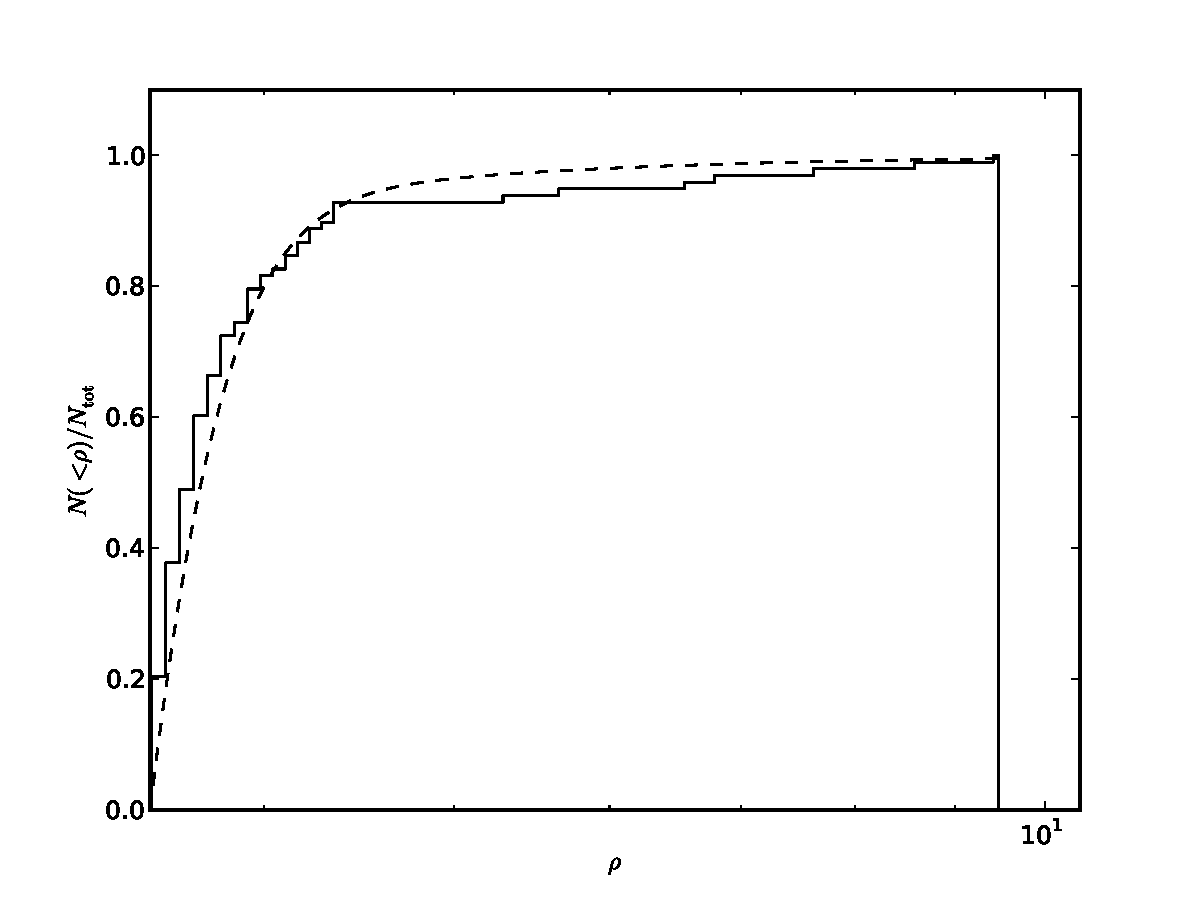
\includegraphics[width=\columnwidth]{data}
  \caption{\label{fig:analytic-data-cumulative} The cumulative
    distribution of the ranking statistics for the synthetic data used
    to test the the formalism on the model from \S
    \ref{sec:analytic-GW-example}.  The solid line gives the
    cumulative distribution of the synthetic data; the dashed line
    gives the theoretical cumulative distribution for the models in
    Eqs.~\eqref{eq:analytic-background-rate} and
    \eqref{eq:analytic-foreground-rate} combined with $R_f = 10.4$ and
    $R_b = 95.1$.}
\end{figure}

In Figure \ref{fig:analytic-rate-recovery}, we show the marginalized
posterior densities for the foreground and background rates.  (Refer
to Eq.~\eqref{eq:rates-marginalized}.)  Figure
\ref{fig:analytic-rate-foreground-probs} shows the posterior
foreground probability for each event marginalized over all other
events' types and the foreground and background rates.  (Refer to
Eq.~\eqref{eq:foreground-marginalized}.)

\begin{figure}
  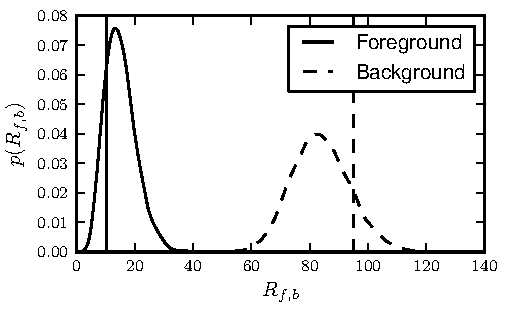
\includegraphics[width=\columnwidth]{rates}
  \caption{\label{fig:analytic-rate-recovery} The posterior densities
    for $R_f$ (in blue) and $R_b$ (in black) for the analytic model
    discussed in \S \ref{sec:analytic-GW-example}.  The vertical lines
    indicate the ``true'' used to generate the synthetic data set.}
\end{figure}

\begin{figure}
  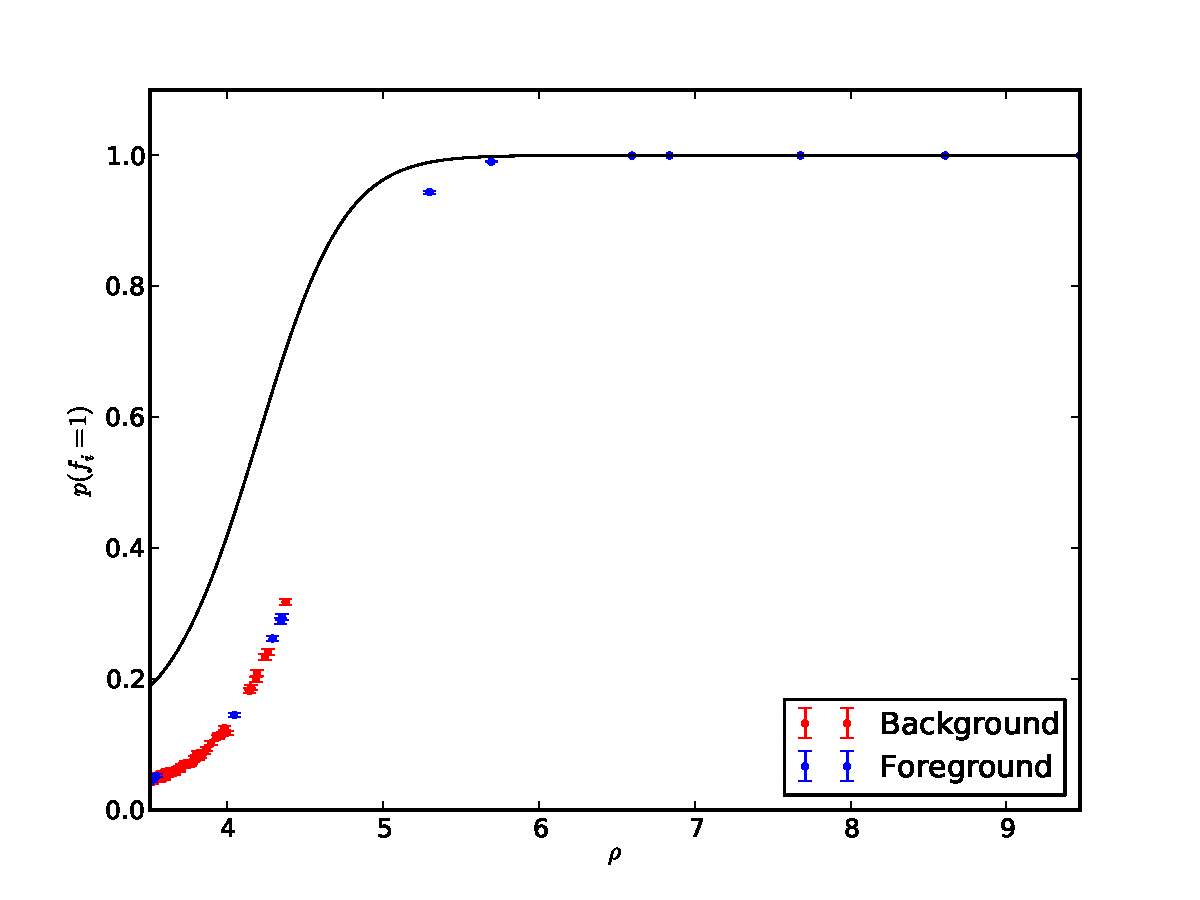
\includegraphics[width=\columnwidth]{pfore}
  \caption{\label{fig:analytic-rate-foreground-probs} Foreground
    probability for each event in the synthetic data set of \S
    \ref{sec:analytic-GW-example} marginalized over all other
    parameters.  True foreground events are in blue, background events
    in red.  The solid line is the likelihood ratio
    $p(x|\mathrm{foreground})/p(x|\mathrm{background})$ (see
    Eq.~\eqref{eq:loudness-likelihood}) for this model; this exceeds
    the marginalized foreground probability for many of the events
    because in this data set there are approximately nine times as
    many background events as foreground events (see
    Eq.~\eqref{eq:foreground-marginalized}). }
\end{figure}

\begin{acknowledgments}
  Kipp Cannon, Chad Hanna, and Drew Keppel for providing the data set
  from \citet{Cannon2012} and assisting us in its use. Richard
  O'Shaughnessy for discussions.
\end{acknowledgments}

\appendix

\section{Likelihood for Inhomogeneous Poisson Processes}
\label{sec:likelihood-derivation}

\fixme{To do.}

%%%%%%%%%%%%%%%%%%%% Bibliography 
\bibliographystyle{apsrev4-1}
\bibliography{many}

\end{document}